\documentclass{standalone}

\usepackage[compat=1.1.0]{tikz-feynman}

\begin{document}

%\feynmandiagram [horizontal=a to b] {
%  i1 [particle=\(e^{-}\)] -- [fermion] a -- [fermion] i2 [particle=\(e^{+}\)],
%  a -- [photon, edge label=\(\gamma\), momentum'=\(k\)] b,
%  f1 [particle=\(\mu^{+}\)] -- [fermion] b -- [fermion] f2 [particle=\(\mu^{-}\)],
%};

%\feynmandiagram [small, horizontal=a to b, tree layout] {
%	
%
%	%a [particle=\(g\)] -- [gluon] b,
%	
%	a [edge label=\(g\)] -- [gluon] b,
%	i1 [particle=\(q\)] -- [fermion] a, 
%	a -- [fermion] i2 [particle=\(\bar{q}\)],
%	
%	b -- [fermion, edge label=\(t\)] c1,
%	c2 -- [fermion, edge label=\(\bar{t}\)] b,
%	
%	c1 -- [fermion] b1 [particle=\(b\)],
%	c1 -- [boson, edge label=\(W^{+}\)] d1, 
%
%	b2 [particle=\(\bar{b}\)] -- [fermion] c2,
%	c2 -- [boson, edge label=\(W^{-}\)] d2,
%
%	l1 [particle=\(l^{+}\)] -- [fermion] d1 -- [fermion] v1 [particle=\(\nu_{l}\)],
%	v2 [particle=\(\bar{\nu}_{l}\)] -- [fermion] d2 -- [fermion] l2 [particle=\(l^{-}\)],
%	
%	{[same layer] i1, i2},
%	{[same layer] c1, c2},
%	{[same layer] d1, d2},
%
%};

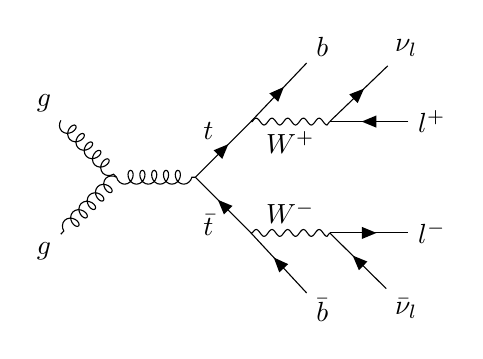
\begin{tikzpicture}
\begin{feynman} [small]
	\vertex (a);
	\vertex [above left=of a] (i1) {\(g\)};
	\vertex [below left=of a] (i2) {\(g\)};
	\vertex [right=of a] (b);
	\vertex [above right=of b] (c1);
	\vertex [below right=of b] (c2);
	
	\vertex [right=of c1] (d1);
	\vertex [right=of c2] (d2);
	\vertex [above right=of c1] (b1) {\(b\)};
 	\vertex [below right=of c2] (b2) {\(\bar{b}\)};
 	
 	\vertex [right=of d1] (l1) {\(l^{+}\)};
 	\vertex [right=of d2] (l2) {\(l^{-}\)};
 	\vertex [above right=of d1] (v1) {\(\nu_{l}\)};
 	\vertex [below right=of d2] (v2) {\(\bar{\nu}_{l}\)};

    \diagram* {

    (a) [edge label=\(g\)] -- [gluon] (b),
	(i1) -- [gluon] (a), 
	(a) -- [gluon] (i2),
	
	(b) -- [fermion, edge label=\(t\)] (c1),
	(c2) -- [fermion, edge label=\(\bar{t}\)] (b),
	
	(c1) -- [fermion] (b1),
	(c1) -- [boson, edge label' =\(W^{+}\)] (d1), 

	(b2) -- [fermion] (c2),
	(c2) -- [boson, edge label =\(W^{-}\)] (d2),

	(l1) -- [fermion] (d1) -- [fermion] (v1),
	(v2) -- [fermion] (d2) -- [fermion] (l2),
    };
\end{feynman}
\end{tikzpicture}

\end{document}